\documentclass{article}
\usepackage[T1]{fontenc}
\usepackage{lmodern}
\usepackage{graphicx}
\usepackage{amsmath,amssymb}
\usepackage[a4paper,margin=2cm]{geometry}
\usepackage[absolute,overlay]{textpos}
\setlength{\TPHorizModule}{1mm}
\setlength{\TPVertModule}{1mm}
\usepackage[indonesian]{babel}
\usepackage{hyperref}
\setlength{\emergencystretch}{2em}
% unit: Halaman 83

\begin{document}

% === Halaman 83 (llm) ===

\begin{itemize}
  \item \textit{Column round} dan \textit{row round} dilakukan di dalam sebuah struktur \textit{quarter round} $\text{QR}(a, b, c, d)$ yang menerima empat \textit{word} sebagai masukan dan menghasilkan empat word luaran:
  
  \begin{align*}
    b & \gets b \oplus (a + d) \lll 7; \\
    c & \gets c \oplus (b + a) \lll 9; \\
    d & \gets d \oplus (c + b) \lll 13; \\
    a & \gets a \oplus (d + c) \lll 18;
  \end{align*}
  
  $\lll k$ adalah pergeseran bit ke kiri sejauh $k$ bit dan bersifat rotasi (siklik)\
  $+$ adalah penjumlahan bit dalam $\bmod 2^{32}$
\end{itemize}

\vspace{20mm}

\textbf{Quarter Round merupakan inti Salsa20}

% deskripsi: Diagram alur operasi Quarter Round yang menunjukkan transformasi variabel a, b, c, dan d menggunakan operasi penjumlahan, rotasi bit (<<<), dan XOR.
% bbox normalisasi: [0.6020, 0.2240, 0.8240, 0.9370]
\begin{textblock*}{46.62mm}(126.42mm,66.53mm)
\noindent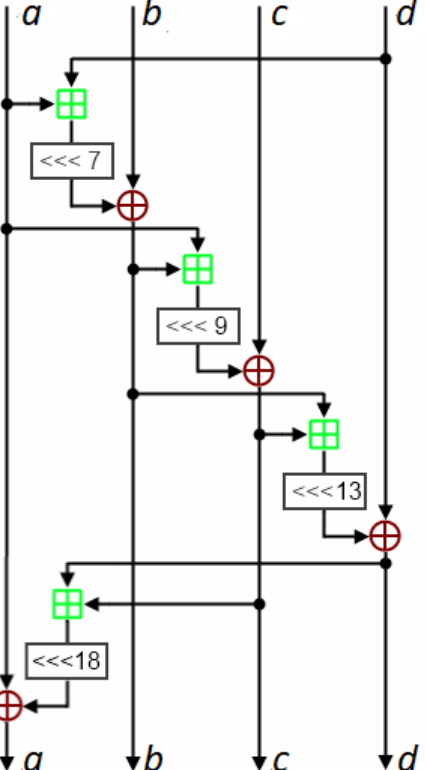
\includegraphics[width=46.62mm,height=211.76mm]{../../images/llm/page_083_img_01.png}%
\end{textblock*}

\end{document}
